\section{Implementation}

This section discusses the implementation of the Carat developer API prototype. The API aims to provide mobile application developers the ability to discover how a client mobile device's system settings and state affect the energy consumption of the device.

The design of such a service poses multiple challenges, as discussed in~\cite{7840871}. The dataset itself is large and incrementally changing as time passes, which makes static statistical analysis inconvenient. It is therefore practical to design the service in such a way that the analysis can be executed dynamically whenever the API is accessed. Another challenge is to protect the privacy of the participants of the Carat project.

Association rules were selected as the basis of the API for two reasons. First, the association rules effectively hide all the details about individual Carat users, protecting their privacy, while also enabling reasonably detailed view on how a devices system settings and state affect the energy consumption. Secondly, efficient parallel algorithms exist for generating association rules from huge datasets as discussed in detail in chapter~\ref{association analysis}.

As discussed in~\cite{7840871}, the intention of the Carat API is to allow application developers to retrieve information about their application by authenticating with their developer key. The prototype described here, does not include authentication of application developers, but rather demonstrates the functionality that the API could offer provided that an authentication has been successfully completed. 

\begin{figure}[!htbp]
	\centering
	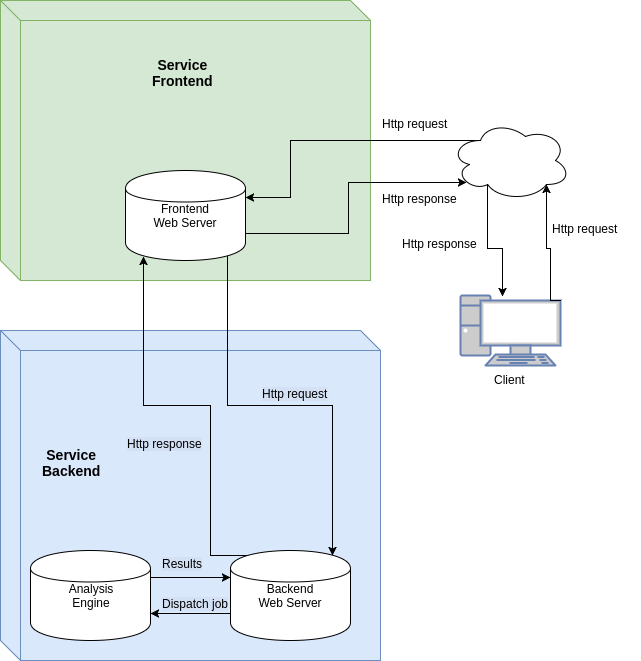
\includegraphics[width=\textwidth]{images/carat-prototype-architecture.png}
	\caption{High level network architecture of the Carat API prototype}
	\label{figure:carat-api-network-prototype}
\end{figure}         

The implementation consists of three main components. These are the front end web server, back end web server and the analysis engine. Figure~\ref{figure:carat-api-network-prototype} shows network level layout of these components and the way these components communicate when the API is accessed. When a client accesses the API, the following flow of requests takes place:
\begin{enumerate}
	\item Client sends a HTTP request to the front end server. The request may contain parameters that control the way the association rules are generated.
	\item Front end web server sends a HTTP request to the back end web server passing along the parameters from the client.
	\item The back end web server dispatches a job to the analysis engine running on SPARK. Parameters provided by the client are used to control the analysis.
	\item Analysis engine sends generated association rules to the back end web server.
	\item Back end server sends HTTP response containing the generated rules to the front end web server.
	\item Front end server uses the association rules to generate a view for the client.  
\end{enumerate}

Figure~\ref{figure:carat-api-network-prototype} shows the flow of control between the different components of the Carat API. The prototype only implements the frontend and the backend of the service. Implementing load balancing and authentication falls outside the scope of this thesis. Some implementation constraints of the authentication module are discussed in~\cite{7840871}.     

\subsection{Service Front End}

\subsection{Service Back End}

The service back end is a simple web server implemented in Scala programming language using Scalatra web framework version 2.4.0. The webserver listens for HTTP GET requests, accepting application name, minimum support, minimum confidence and a list variable names to be excluded in the requests URL parameters. Once a valid GET request is received, the server creates a Spark job script based on the request parameters, and submits the Spark job to the analysis engine. The shell script which submits the Spark job is executed in a thread pool asynchronously to avoid making the web server unresponsive while a Spark job is running. Once the analysis engine has successfully executed the job, the shell script prints the association rules in JSON format to its standard output stream. This output is captured and returned as a HTTP response to the client.

The server consists of merely three components, a servlet, a service and a bootstrap component. The bootstrap components purpose in Scalatra is to mount services to certain URL paths. The bootstrap component simply mounts our servlet to match with any path, as denoted by asterisk character 
\begin{minipage}{\linewidth}
\begin{lstlisting}[language=scala]
class ScalatraBootstrap extends LifeCycle {
  override def init(context: ServletContext) {
    context.mount(new MainServlet, "/*")
  }
}
\end{lstlisting}
\end{minipage}   

A servlet is a server component that routes incoming requests to associated controller routines. The servlet in question is implemented is Scalatra as follows

\begin{minipage}{\linewidth}
\begin{lstlisting}[language=scala]
class MainServlet extends ScalatraServlet with FutureSupport with JacksonJsonSupport {

  val conf = ConfigFactory.load()
  override val asyncTimeout = conf.getInt("timeout") seconds
  protected implicit lazy val jsonFormats: Formats = DefaultFormats
  implicit val executor = ExecutionContext.global
  
  before() {
    contentType = formats("json")
  }
	
  get("/") {
    val applicationName = Try(params("applicationName")).toOption
	val minSupport = Try(params("minSupport").toDouble).toOption
	val minConfidence = Try(params("minConfidence").toDouble).toOption
    val excluded = Try(params("excluded")).toOption.getOrElse("")

    applicationName.map { applicationName =>
      SparkRunner.runSpark(
        applicationName,
        minSupport = minSupport,
        minConfidence = minConfidence,
        excluded = excluded
      )
    }.getOrElse {
      BadRequest(reason = "Missing 'applicationName'")
    }
  }
}
\end{lstlisting}
\end{minipage}  

The traits \textit{FutureSupport} and \textit{JacksonJsonSupport} indicate, that the response is computed asynchronously and is JSON formatted. The method call to \textit{get("/")} registers a controller routine to the root path of the servlet. The controller routine, which is given as a call-by-name function to the second parameter list of the \textit{get} call, parses URL parameters from the incoming HTTP request and submits a new task to the \textit{SparkRunner} service. In case the \textit{applicationName} is missing from the request, a \textit{BadRequest} HTTP response is produced, otherwise the service method \textit{runSpark} is executed asynchronously and a response will be sent once the analysis engine has accomplished its analysis. For example, suppose that the server is running on localhost and listening on port 8888. Upon receiving a GET request to an URI such as \textit{localhost:8888?applicationName=com.facebook.katana\&minConfidence=0.9}, the servlet would route the request to the controller routine configured under \textit{get("/")}. The routine would parse the URI parameters \textit{applicationName} and \textit{minConfidence} and dispatch a Spark job to the analysis engine by invoking \textit{SparkRunner.runSpark}.  



\subsection{Analysis Engine}

\begin{wrapfigure}{r}{0.35\textwidth}
	\vspace{-110pt}
	\begin{center}
		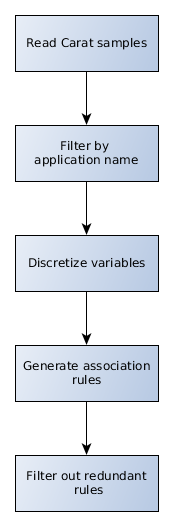
\includegraphics[width=0.3\textwidth]{images/analysis_engine_flow_graph.png}
	\end{center}
	\caption{Overview of the analysis engine pipeline}
	\label{figure:analysis-engine-flow-graph}
\end{wrapfigure}

The primary function of the analysis engine is to generate association rules from the Carat data based on provided query parameters. The query parameters consist of application name, minimum confidence, minimum support and an optional list of attribute names which are to be excluded from the analysis. The application name is used to filter out all Carat energy rate samples in which the the application is not present. The minimum support and minimum confidence parameters affect the association rule generation as described in chapter~\ref{association analysis}. The excluded attributes list controls the association rule generation by completely ignoring all included attributes.    

%\begin{figure}[!htbp]
%	\centering
%	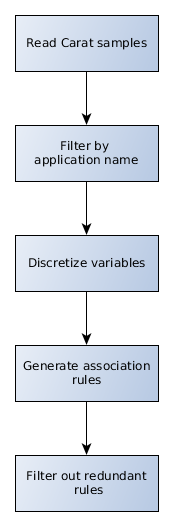
\includegraphics[width=0.25\textwidth]{images/analysis_engine_flow_graph.png}
%	\caption{Overview of the analysis engine pipeline}
%	\label{figure:analysis-engine-flow-graph}
%\end{figure}    
 
Figure~\ref{figure:analysis-engine-flow-graph} describes the process of generating association rules as a simple pipeline consisting of four steps. We will now go through each step providing snippets of code, taken from the analysis engine implementation, that will shed light on the implementation in Spark programming framework. 

Reading Carat samples is very simple in Spark, as is evident from the following code snippet.  

\begin{minipage}{\linewidth}
\begin{lstlisting}[language=scala]
def readCaratRates(sampleDir: String)(implicit sc: SparkContext): RDD[fi.helsinki.cs.nodes.carat.sample.Rate] = {
	sc.objectFile[fi.helsinki.cs.nodes.carat.sample.Rate](s"${sampleDir}")
}
\end{lstlisting}
\end{minipage}

The $objectFile$ method of the $SparkContext$ object will read the dataset from a given directory. The dataset is stored as an RDD (Resilient Distributed Dataset), that is serialized to the disk in a folder given by the $sampleDir$ parameter. RDD is is the data structure that Spark framework uses to store, access and transform distributed datasets. The Carat samples are initially read as instances of class $fi.helsinki.cs.nodes.carat.sample.Rate$. Each $Rate$ object contains two consecutive samples from a mobile device. From these samples, the system settings and running mobile applications can be extracted as described in chapter~\ref{carat data}  

The next task that the analysis engine carry out, is to filter out all Carat rate samples where the requested application was not running. Using the $readCaratRates$ method, one can compose an expression which reads Carat rate data objects, filters out all rate objects that do not have the requested application running and transforms the resulting rate objects to a simplified object type of class $Sample$. 

\begin{minipage}{\linewidth}
\begin{lstlisting}[language=scala]
val samples = readCaratRates(ratePath).collect {
	case rate if rate.allApps().contains(applicationName) => 
		Sample.fromCaratRate(rate)
}
\end{lstlisting}
\end{minipage}  
The $collect$ is a method defined for all instances of class $RDD[T]$ (where $T$ is a type parameter). It is analogous to the $collect$ method from Scala standard library, taking a partial function of signature $PartialFunction[T, U]$  (where $T$ and $U$ are type parameters) and returning a new instance of $RDD[U]$, containing the image of the $RDD[T]$ mapped by the partial function.
        
The $Sample$ is a simple case class that merely stores all the relevant system settings. The case class also has a companion object, in which the method $fromCaratRate$ is defined. The method simply constructs a $Sample$ instance from a $Rate$ instance. 

\begin{minipage}{\linewidth}
\begin{lstlisting}[language=scala]
case class Sample(
	rate: Double,
	cpu: Double,
	distance: Double,
	temp: Double,
	voltage: Double,
	screen: Double,
	mobileNetwork: String,
	network: String,
	wifiStrength: Double,
	wifiSpeed: Double
)
\end{lstlisting}
\end{minipage}  

The next step in the analysis work flow, is to discretize the variables of the data. All numerical variables were discretized to bins of equal mass, as explained in depth in chapter~\ref{carat data}. The following code snippet shows how to find the break points of the bins for continuously valued variables.

\begin{minipage}{\linewidth}
\begin{lstlisting}[language=scala] 
def getQuantiles(
  data: RDD[Double],
  buckets: Int,
  relativeError: Double = 0.0001,
  partial: 
  	PartialFunction[Double, Option[String]] = Map.empty)
  (implicit sqlContext: SQLContext): 
Array[Double] = {
	
  import sqlContext.implicits._

  val percentiles = (for(i <- 1 to (buckets - 1)) yield (1.0 / buckets) * i).toArray
  val notDefined = data.filter(x => !partial.isDefinedAt(x))

  try {
    notDefined.toDF("col").stat.approxQuantile("col", percentiles, relativeError)
  } catch{
    case ex: java.util.NoSuchElementException => Array[Double]()
  }
}
\end{lstlisting}
\end{minipage}  

The method $getQuantiles$ takes as an its input $data$, an $RDD$ containing the values to be discretized; $buckets$, the number of bins to create; $relativeError$, the maximum relative error that is allowed when approximating the break points of the percentiles; $partial$, a partial function that is used to filter out values that should not be taken into account when approximating the percentiles. The method uses Spark $DataFrame$ API to approximate the percentiles. Using a $relativeError$ parameter larger than 0, makes the generation of the association rules non deterministic, since the approximated percentile break points are allowed to vary from the exact value. However, calculating exact values for the breakpoints (by setting the $relativeError$ parameter to zero) slows down the generation of the association rules considerably, as all of the data needs to be processed in order to calculate the break points as opposed to calculating the break points from a sampled dataset.

Having computed the quantiles of a continuously valued variable, discretization can be achieved by using the following method

\begin{minipage}{\linewidth}
\begin{lstlisting}[language=scala] 
def getFeatureFromQuantiles(
	dataPoint: Double,
	featureName: String,
	quantiles: Array[Double],
	partial: PartialFunction[Double, Option[String]] = Map.empty
): Option[String] = {
	if(partial.isDefinedAt(dataPoint))
		return partial(dataPoint).map { x => 
			s"${featureName}=${x}"
		}
	
	var index = quantiles.indexWhere(q => q >= dataPoint) + 1	
	if (index == 0) index += (quantiles.length + 1)
	Some(s"${featureName}=q${index}")
}  
\end{lstlisting}
\end{minipage}  

The method \textit{getFeaturesFromQuantiles} takes as its input \textit{dataPoint}, a single point of data to be discretized; \textit{featureName}, the name of the feature; \textit{quantiles}, the quantile break points for the variable and \textit{partial} a partial function that is used both to filter out invalid data as well as to bypass the discretization altogether.

As a concrete example, let us examine how one could go about discretizing variable \textit{screen}, which gives the screen brightness of the mobile device. As discussed in chapter~\ref{carat data screen}, the variable takes values between -1 and 255, where value -1 signifies a special case, where the screen brightness is automatically adapted to the brightness of the surroundings of the device. One could encode these preconditions to a partial function of the following form:
\begin{minipage}{\linewidth}
\begin{lstlisting}[language=scala] 
val screenPartial: PartialFunction[Double, Option[String]] = {
    case x if x == -1 => Some("auto")
    case x if x < -1 => None
	case x if x > 255 => None
}
\end{lstlisting}
\end{minipage} 
Using this partial function in conjunction with the methods \textit{getQuantiles} and \textit{getFeatureFromQuantiles} for each data point will give the discretized form of the variable \textit{screen}. 

To summarise: in order to discretize a variable such as \textit{screen}, which is assumed to be a collection of type \textit{RDD[Double]}, one could fist calculate the quantiles of data using the method \textit{getFeatureFromQuantiles}. One must then define a partial function, such as the one mentioned above, that filters out invalid data points and handles values with special significance. Finally, the method \textit{getFeatureFromQuantiles} could be applied to each data point of the collection using the partial function and the quantiles.

Having ediscretized all the variables of the dataset, using the procedure discussed above, one ends up with one array of strings for each sample, which is represented in Spark by type \textit{RDD[Array[String]]}. To generate the association rules from these discrete features, MLlib, a machine learning library for Spark was used. The library implements a parallel FPGrowth algorithm for this purpose. The FPGrowth implementation has a limitation however, in that it can only generate rules with single consequent. The limitation is not terribly severe for the purpose of this thesis, as the main interest lies in finding out which variables affect the battery usage. Therefore being limited to rules which have as their sole consequent a feature extracted from the energy rate variable, should be sufficient. The following snippet of code illustrates how to generate association rules using the MLlib API.

\begin{minipage}{\linewidth}
\begin{lstlisting}[language=scala] 
val fpg = new FPGrowth()
		  .setMinSupport(minSupport)
			  
val model = fpg.run(features)

val rulesFiltered = model.generateAssociationRules(minConfidence)
  .filter { rule =>
    rule.consequent.find { item =>
	  item.startsWith("rate=")
	}.isDefined
  }
\end{lstlisting}
\end{minipage}       

The final stage of association rule generation workflow is filtering out redundant rules. To demonstrate what is meant by redundancy in this context, let us consider two rules such as    

\begin{equation}
	\left\{ A, B \right\}  \Rightarrow  \left\{ X \right\} \label{rule:1}
\end{equation}

\begin{equation}
\left\{ A, B, C \right\}  \Rightarrow  \left\{ X \right\} \label{rule:2}
\end{equation}

Additionally, let us assume that both rules \eqref{rule:1} and \eqref{rule:2} have equivalent confidence. Since both rules predict the same consequents and the antecedents of rule \eqref{rule:1} is a subset of the antecedents of rule \eqref{rule:2}, one can conclude that the rule \eqref{rule:1} is the more general of the two rules, as adding item \textit{C} to the antecedents of rule \eqref{rule:1} does not improve the associative power of the original rule. Since the objective of this thesis is to identify variables which have the strongest association with the battery consumption of a mobile application, we consider rule \eqref{rule:2} redundant in the context of this thesis work.

More generally, given a set \textit{S} of association rules, we consider rule $R \in S$ redundant if there exists a rule $r \in S$, such that $R \neq r$ and $r.antedecents \subset R.antedecents$. The following excerpt of code shows how this definition translates to a redundancy filtering algorithm in Scala programming language
    
    \begin{minipage}{\linewidth}
\begin{lstlisting}[language=scala] 
def pruneRules(rules: RDD[Rule[String]]): RDD[Rule[String]] = {
  val pruneCandidateGroups = rules.groupBy{ rule => 
    (rule.consequent.sorted.mkString, rule.confidence) 
  }

  pruneCandidateGroups.flatMap { case (key, group) =>
    val groupSorted = group.toSeq.sortBy(rule => rule.consequent.length)
    var groupAsSets = group.map(rule => (rule, rule.antecedent.toSet))

    val toPrune: Set[Rule[String]] = (for {
      testRule <- groupAsSets
      otherRule <- groupAsSets
      if testRule != otherRule && testRule._2.subsetOf(otherRule._2)
    } yield(otherRule._1)).toSet
    
    groupSorted.filter(rule => !toPrune.contains(rule))
  }
}
\end{lstlisting}
\end{minipage}       

Method \textit{pruneRules} takes a collection of association rules and returns a collection of association rules which contains no redundant rules.

This concludes the analysis engine part of the implementation. From usability perspective, generating the association rules should be fast enough not to hinder interactive use, which implies that the rule generation should not take more than a couple of seconds. However, heavily optimizing the analysis engine falls outside the scope of this thesis. In practice, the implementation described here achieves run times of a couple of minutes with a rather modest dataset size of 16 gigabytes. In practice, 


   